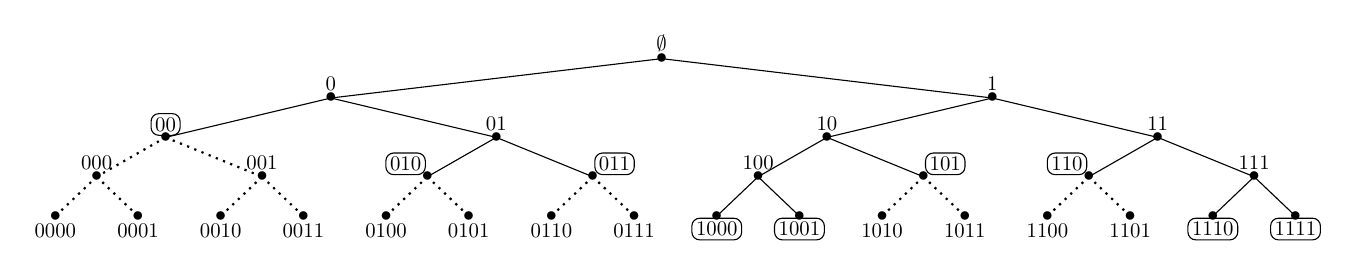
\begin{tikzpicture}[xscale=1.4]
\shorthandoff{>}
%
% nivel 2^4
%%%%%%%%%%%%
\draw[thick,dotted] (.375,.5)--(0,0) node[scale=.8]{$\bullet$} node[below,scale=.75]{0000};
\draw[thick,dotted] (.375,.5)--(.75,0) node[scale=.8]{$\bullet$} node[below,scale=.75]{0001};
\draw[thick,dotted] (1.875,.5)--(1.5,0) node[scale=.8]{$\bullet$} node[below,scale=.75]{0010};
\draw[thick,dotted] (1.875,.5)--(2.25,0) node[scale=.8]{$\bullet$} node[below,scale=.75]{0011};
\draw[thick,dotted] (3.375,.5)--(3,0) node[scale=.8]{$\bullet$} node[below,scale=.75]{0100};
\draw[thick,dotted] (3.375,.5)--(3.75,0) node[scale=.8]{$\bullet$} node[below,scale=.75]{0101};
\draw[thick,dotted] (4.875,.5)--(4.5,0) node[scale=.8]{$\bullet$} node[below,scale=.75]{0110};
\draw[thick,dotted] (4.875,.5)--(5.25,0) node[scale=.8]{$\bullet$} node[below,scale=.75]{0111};
%
\draw (6.375,.5)--(6,0) node[scale=.8]{$\bullet$}
node[inner sep=2pt,outer sep=1pt,draw=black,below,scale=.75,rounded corners=1mm]{1000};
%
\draw (6.375,.5)--(6.75,0) node[scale=.8]{$\bullet$}
node[inner sep=2pt,outer sep=1pt,draw=black,below,scale=.75,rounded corners=1mm]{1001};
%
\draw[thick,dotted] (7.875,.5)--(7.5,0) node[scale=.8]{$\bullet$} node[below,scale=.75]{1010};
\draw[thick,dotted] (7.875,.5)--(8.25,0) node[scale=.8]{$\bullet$} node[below,scale=.75]{1011};
\draw[thick,dotted] (9.375,.5)--(9,0) node[scale=.8]{$\bullet$} node[below,scale=.75]{1100};
\draw[thick,dotted] (9.375,.5)--(9.75,0) node[scale=.8]{$\bullet$} node[below,scale=.75]{1101};
%
\draw (10.875,.5)--(10.5,0) node[scale=.8]{$\bullet$}
node[inner sep=2pt,outer sep=1pt,draw=black,below,scale=.75,rounded corners=1mm]{1110};
%
\draw (10.875,.5)--(11.25,0) node[scale=.8]{$\bullet$}
node[inner sep=2pt,outer sep=1pt,draw=black,below,scale=.75,rounded corners=1mm]{1111};
%
%----------
%
% nivel 2^3
%%%%%%%%%%%%
\draw[thick,dotted] (1,1)--(.375,.5) node[scale=.8]{$\bullet$} node[above,scale=.75]{000};
\draw[thick,dotted] (1,1)--(1.875,.5) node[scale=.8]{$\bullet$} node[above,scale=.75]{001};
%
\draw (4,1)--(3.375,.5) node[scale=.8]{$\bullet$}
node[inner sep=2pt,outer sep=1pt,draw=black,above left,scale=.75,rounded corners=1mm]{010};
%
\draw (4,1)--(4.875,.5) node[scale=.8]{$\bullet$}
node[inner sep=2pt,outer sep=1pt,draw=black,above right,scale=.75,rounded corners=1mm]{011};
%
\draw (7,1)--(6.375,.5) node[scale=.8]{$\bullet$} node[above,scale=.75]{100};
%
\draw (7,1)--(7.875,.5) node[scale=.8]{$\bullet$}
node[inner sep=2pt,outer sep=1pt,draw=black,above right,scale=.75,rounded corners=1mm]{101};
%
\draw (10,1)--(9.375,.5) node[scale=.8]{$\bullet$}
node[inner sep=2pt,outer sep=1pt,draw=black,above left,scale=.75,rounded corners=1mm]{110};
%
\draw (10,1)--(10.875,.5) node[scale=.8]{$\bullet$} node[above,scale=.75]{111};
%
%----------
%
% nivel 2^2
%%%%%%%%%%%%
\draw (2.5,1.5)--(1,1) node[scale=.8]{$\bullet$}
node[inner sep=2pt,outer sep=1pt,draw=black,above,scale=.75,rounded corners=1mm]{00};
%
\draw (2.5,1.5)--(4,1) node[scale=.8]{$\bullet$} node[above,scale=.75]{01};
\draw (8.5,1.5)--(7,1) node[scale=.8]{$\bullet$} node[above,scale=.75]{10};
\draw (8.5,1.5)--(10,1) node[scale=.8]{$\bullet$} node[above,scale=.75]{11};
%
%----------
%
% nivel 2^1
%%%%%%%%%%%%
\draw (5.5,2)--(2.5,1.5) node[scale=.8]{$\bullet$} node[above,scale=.75]{0};
\draw (5.5,2)--(8.5,1.5) node[scale=.8]{$\bullet$} node[above,scale=.75]{1};
%
%----------
%
% nivel 2^0
%%%%%%%%%%%%
\draw (5.5,2) node[scale=.8]{$\bullet$} node[above,scale=.75]{$\emptyset$};

\end{tikzpicture}